\documentclass[a4paper,12pt]{report}

\usepackage{alltt, fancyvrb, url}
\usepackage{graphicx}
\usepackage[utf8]{inputenc}
\usepackage{float}
\usepackage{xcolor}
\usepackage{hyperref}

% Questo commentalo se vuoi scrivere in inglese.
\usepackage[italian]{babel}

\usepackage[italian]{cleveref}

\title{Meta-relazione per\\``Programmazione ad Oggetti''}

\author{Filippo Greppi, Elena Fucci, Spaccini Ettore}
\date{\today}


\begin{document}

\maketitle

\begin{abstract}
 %%

\end{abstract}

\tableofcontents

\chapter{Analisi}

\section{Descrizione e requisiti}
Il software mira allo sviluppo del videogioco “Mind-Escape”, un’avventura psicologica e di suspense. Il giocatore assume il ruolo di un personaggio che si sveglia in una stanza sconosciuta, senza memoria di come ci sia arrivato. L’obiettivo del gioco è fuggire da questa prigionia, risolvendo una serie di enigmi che si presentano in diverse stanze. Ogni enigma risolto porta il giocatore più vicino alla vittoria, aprendo la via verso la stanza successiva.
%
Per avanzare, il giocatore deve raccogliere e utilizzare vari oggetti, che vengono gestiti attraverso un inventario. Questi oggetti sono essenziali per risolvere enigmi e accedere a nuove stanze.
%
La partita si concluderà quando il giocatore raggiungerà e risolverà l’enigma finale, riuscendo a fuggire dall’ultima stanza.
%

\subsubsection{Requisiti funzionali}
\begin{itemize}
	\item Il personaggio deve poter muoversi nella mappa, gestendo le collisioni con ostacoli e pareti
	\item Il gioco deve permettere al personaggio di interagire con gli oggetti nelle stanze (es. raccogliere, esaminare, usare).
	\item Il personaggio deve disporre di un inventario che permetta di gestire gli oggetti raccolti.
	\item Il sistema deve verificare automaticamente la correttezza delle soluzioni degli enigmi.
\end{itemize}

\subsubsection{Requisiti non funzionali}
\begin{itemize}
	\item Salvataggio dello stato della partita
	\item Deve essere garantita una modularità del codice per consentire l'aggiunta futura di nuove stanze o enigmi.
	\item Ridimensionabilità della finestra di gioco
\end{itemize}

\section{Modello del Dominio}

Mind Escape è un gioco ambientato in un mondo suddiviso in più stanze, attraverso le quali il giocatore può muoversi ed interagire con vari oggetti. 
L’avventura ha inizio in una stanza iniziale, da cui il giocatore potrà accedere progressivamente alle altre stanze. 
Il passaggio tra le stanze avviene mediante porte, che possono essere sbloccate risolvendo enigmi o utilizzando oggetti raccolti durante il gioco. L'obiettivo finale è raggiungere l’ultima stanza e interagire con uno specifico oggetto, evento che determina la vittoria.

\begin{figure}[h]  % [h] indica che la figura sarà posizionata il più vicino possibile
    \centering
    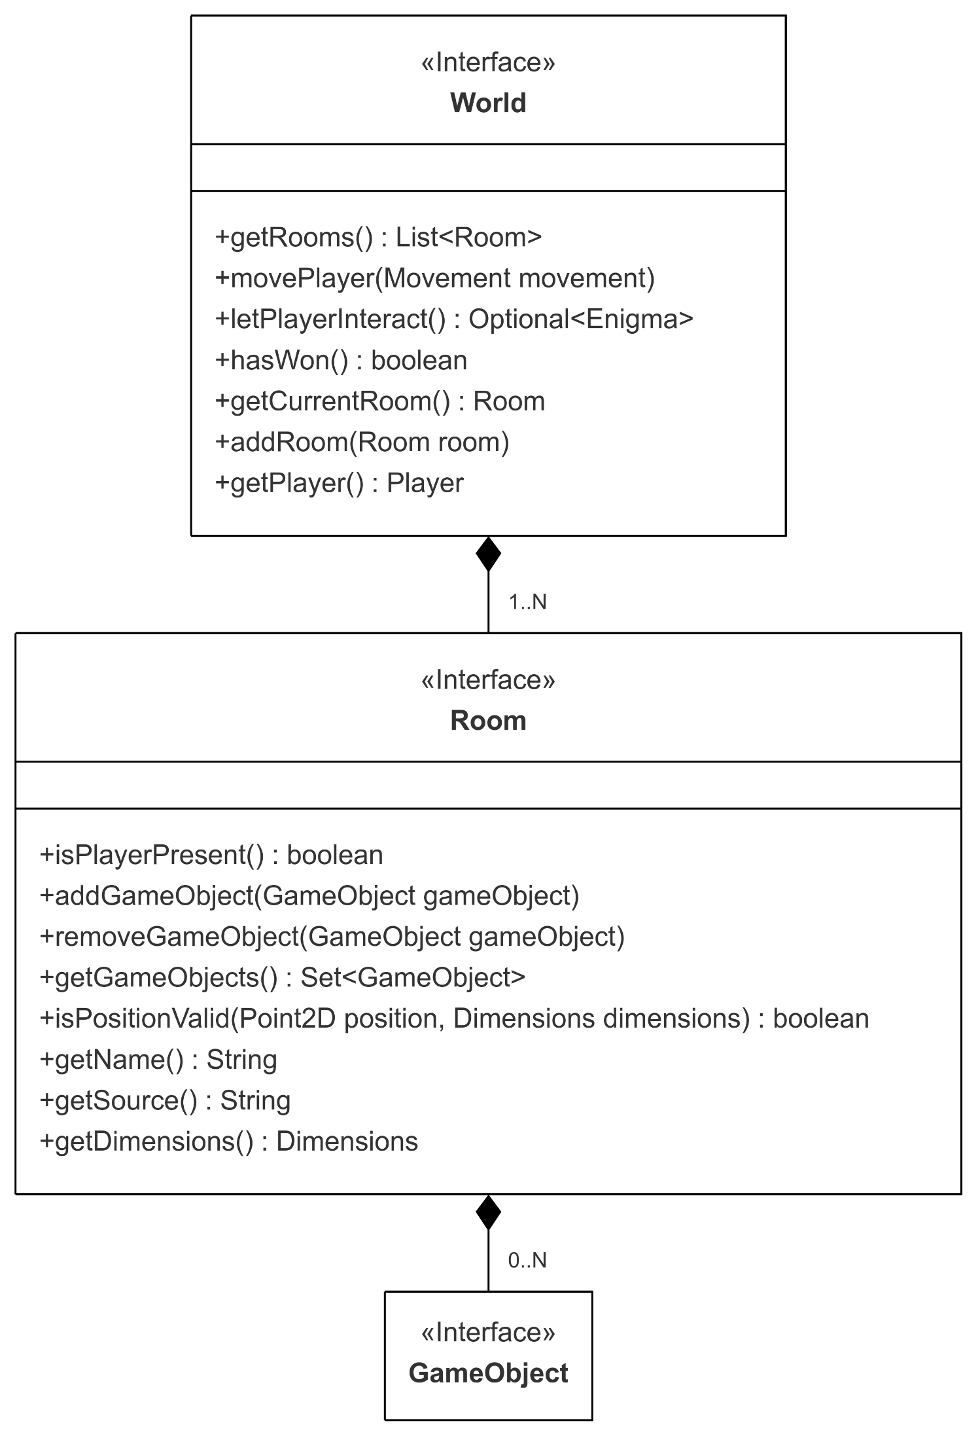
\includegraphics[width=0.8\textwidth]{img/model.png}  % Modifica width se serve
    \caption{Esempio di game object}
    \label{img:gameObject}
\end{figure}

All'interno di ogni stanza possono essere presenti oggetti di gioco (GameObject), con i quali il giocatore può collidere. 
Gli oggetti di gioco si suddividono in due categorie principali:
\begin{itemize}
	\item Oggetti interagibili (Interactable): si distinguono in due sottocategorie:
	\begin{itemize}
		\item Oggetti raccoglibili (Pickable): possono essere raccolti dal giocatore ed inseriti nell’inventario, dove potranno essere utilizzati successivamente.
		\item Oggetti non raccoglibili (Unpickable): non possono essere raccolti, ma possono essere sbloccati tramite determinate azioni. Alcuni di essi possono essere associati alla risoluzione di un enigma.
	\end{itemize}
	L'interazione tra il giocatore e un oggetto interagibile può avvenire esclusivamente a seguito di una collisione. In seguito all'interazione, l'oggetto esegue un'azione predefinita che determina il suo comportamento e le conseguenze dell'interazione.
	\item Oggetti non interagibili (NonInteractable): questi oggetti hanno una funzione puramente estetica o di ambientazione, e non influenzano direttamente il gameplay. Tuttavia, il giocatore può collidere con essi.
\end{itemize}

\begin{figure}[h]  % [h] indica che la figura sarà posizionata il più vicino possibile
    \centering
    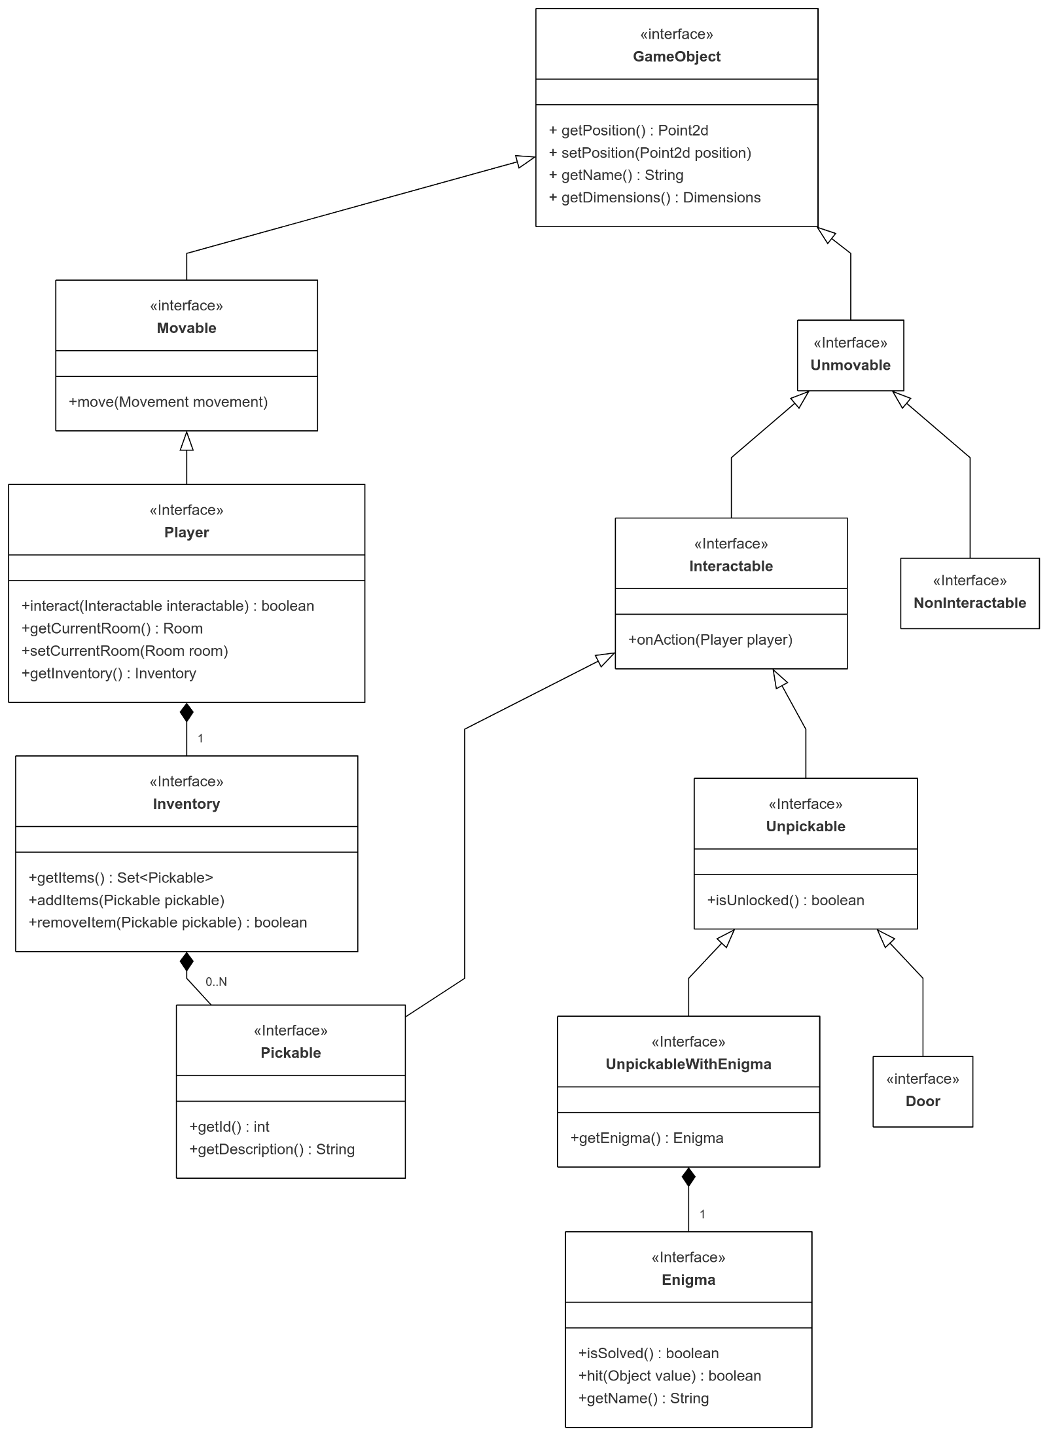
\includegraphics[width=0.8\textwidth]{img/gameObject.png}  % Modifica width se serve
    \caption{Esempio di game object}
    \label{img:gameObject}
\end{figure}
 % 
\chapter{Design}
\section{Architettura}
L'architettura di Mind-Escape segue il pattern architetturale MVC (Model-View-Controller), ma si compone di più strutture MVC modulari. 
Il sistema implementa un'interfaccia chiamata MainController, che ha il compito di cercare e attivare i controller appropriati in base alle azioni dell'utente. 
I controller disponibili sono quelli associati ai vari MVC, e sono suddivisi in due categorie principali:
\begin{itemize}
	\item LoopController: Gestisce gli MVC che richiedono un aggiornamento costante sia dal punto di vista logico che grafico. L'esecuzione di questi aggiornamenti può essere avviata o interrotta in base alle decisioni del MainController.
	\item 2.	ClickableController: Gestisce gli MVC che necessitano di un aggiornamento sia logico che grafico, ma solo in seguito a un'interazione esplicita dell'utente, come l'uso del mouse o la tastiera.
\end{itemize}
%
Ogni controller è in grado di notificare il MainController riguardo al passaggio al controller successivo. Il MainController è responsabile della creazione e gestione dei controller necessari, ottimizzando l'uso della memoria in base alle esigenze specifiche. 
Questo approccio consente di aggiungere un numero arbitrario di controller senza compromettere la struttura dell'applicazione.
%
Inoltre, Mind-Escape supporta la registrazione di input e output all'interno delle view di ciascun MVC.
Gli input rappresentano nuove informazioni inviate ai controller, che possono includere comandi da mouse, tastiera, o l'inserimento di password. 
Questi input sono generati dall'utente e possono scatenare eventi che modificano il controller corrente. Una volta ricevuti gli input, il MainController aggiorna la view corretta in output, permettendo un'interazione dinamica e fluida.
%
In sintesi, l'aggiunta di nuovi Model, Controller e View non richiede modifiche alla struttura centrale dell'applicazione, garantendo così una scalabilità e una modularità efficaci.
%

\begin{figure}[h]  % [h] indica che la figura sarà posizionata il più vicino possibile
    \centering
    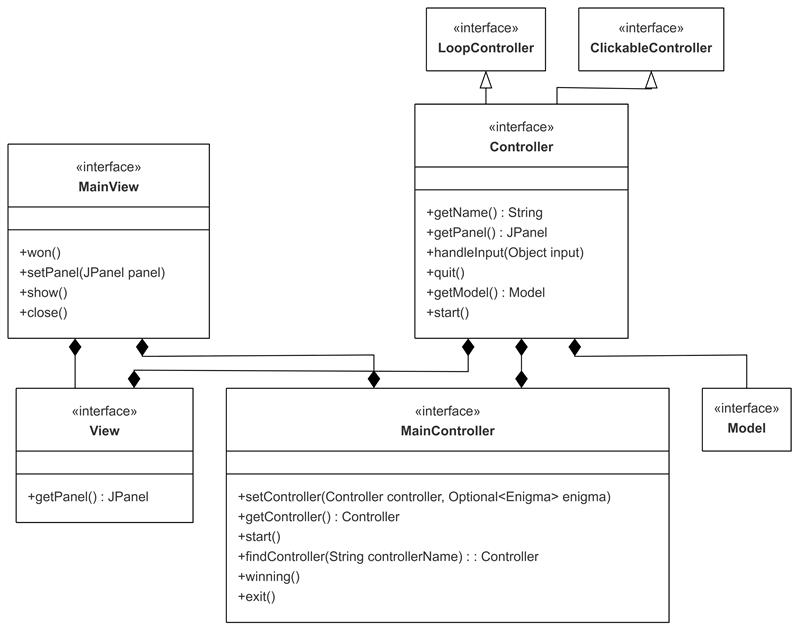
\includegraphics[width=0.8\textwidth]{img/mvc.png}  % Modifica width se serve
    \caption{Esempio di game object}
    \label{img:gameObject}
\end{figure}

% arrivato qui
\section{Design dettagliato}
%% forse va messo la descrizione
\subsection{Elena Fucci}
%
\paragraph{Problema} %%descrizione del problema
\paragraph{Soluzione} %% descrizione della soluzione
%
\subsection{Filippo Greppi}
%
\paragraph{Problema} %%descrizione del problema
\paragraph{Soluzione} %% descrizione della soluzione
%
\subsection{Ettore Spaccini}
%
\paragraph{Problema} %%descrizione del problema
\paragraph{Soluzione} %% descrizione della soluzione

%
\subsection{Marcello Spagnoli}
%
\paragraph{Problema} %%descrizione del problema
\paragraph{Soluzione} %% descrizione della soluzione
%


\chapter{Sviluppo}
\section{Testing automatizzato}

\begin{itemize}
	\item 
	% inserire quali test sono stati fatti e come sono stati fatti

\end{itemize}




\section{Note di sviluppo}

% qui vanno inseriti i permalink

\chapter{Commenti finali}


\section{Autovalutazione e lavori futuri}

%
Ciascuno dovrà autovalutare il proprio lavoro, elencando i punti di forza e di debolezza in quanto prodotto.
Si dovrà anche cercare di descrivere \emph{in modo quanto più obiettivo possibile} il proprio ruolo all'interno del gruppo.
Si ricorda, a tal proposito, che ciascuno studente è responsabile solo della propria sezione: non è un problema se ci sono opinioni contrastanti, a patto che rispecchino effettivamente l'opinione di chi le scrive.
Nel caso in cui si pensasse di portare avanti il progetto, ad esempio perché effettivamente impiegato, o perché sufficientemente ben riuscito da poter esser usato come dimostrazione di esser capaci progettisti, si descriva brevemente verso che direzione portarlo.

\section{Difficoltà incontrate e commenti per i docenti}

Questa sezione, \textbf{opzionale}, può essere utilizzata per segnalare ai docenti eventuali problemi o difficoltà incontrate nel corso o nello svolgimento del progetto, può essere vista come una seconda possibilità di valutare il corso (dopo quella offerta dalle rilevazioni della didattica) avendo anche conoscenza delle modalità e delle difficoltà collegate all'esame, cosa impossibile da fare usando le valutazioni in aula per ovvie ragioni.
%
È possibile che alcuni dei commenti forniti vengano utilizzati per migliorare il corso in futuro: sebbene non andrà a vostro beneficio, potreste fare un favore ai vostri futuri colleghi.
%
Ovviamente \textit{il contenuto della sezione non impatterà il voto finale}.

\appendix
\chapter{Guida utente}

I comandi di gioco sono i seguenti:
\begin{itemize}
	\item \textbf{W, A, S, D}: per muovere il personaggio
	\item \textbf{E}: per interagire con gli oggetti
	\item \textbf{I}: per aprire l'inventario
\end{itemize}

\chapter{Guida soluzione}
%
\section{Stanza 1 - Camera da Letto}
\begin{itemize}
	\item Interagendo con letto si raccoglie un biglietto 
	\item Interagendo con il tavolo si apre un puzzle 
	\item la porta si sblocca inserendo la password “Sergio Mattarella”
\end{itemize}
%
\section{Stanza 2 - Mensa}
\begin{itemize}
	\item Raccogliere il biglietto sul tavolo 
	\item Guardare il calendario (vicino alla porta di entrata) come suggerisce il biglietto 
	\item Interagire con la cassettiera vicino al calendario (Password: “12-13”) 
	\item Interagire di nuovo con la cassettiera per prendere la chiave (che sblocca una delle due porte) 
	\item Raccogliere la chiave inglese  
	\item Provare a sbloccare una delle 2 porte
\end{itemize}
%
\section{Stanza 3 - Ufficio}
\begin{itemize}
	\item Raccogliere la torcia 
	\item Interagire col computer (Shift: “3”) 
	\item Tornare alla mensa 
	\item Tentare di sbloccare la porta rimasta 
\end{itemize}
%
\section{Stanza 4 - Archivio}
\begin{itemize}
	\item Aprire la cassa raccogliendo il martello
	\item Andare nell’ armadio in mezzo alla stanza e inserire la password del cifrario: “oblivion” 
	\item Interagire di nuovo con l’armadio per prendere il biglietto al suo interno (che sblocca l’ultima porta) 
\end{itemize}
%
\section{Stanza 5 - Finale}
\begin{itemize}
	\item Interagire con lo specchio
\end{itemize}

\appendix
\chapter{Esercitazioni di laboratorio}

 
\subsection{paperon.depaperoni@studio.unibo.it} % email di chi lo ha fatto

\begin{itemize}
 \item Laboratorio 04: \url{https://virtuale.unibo.it/mod/forum/discuss.php?d=12345#p123456}
 \item Laboratorio 05: \url{https://virtuale.unibo.it/mod/forum/discuss.php?d=22222#p222222}
 \item Laboratorio 06: \url{https://virtuale.unibo.it/mod/forum/discuss.php?d=99999#p999999}
 \item Laboratorio 07: \url{https://virtuale.unibo.it/mod/forum/discuss.php?d=22222#p222222}
 \item Laboratorio 08: \url{https://virtuale.unibo.it/mod/forum/discuss.php?d=99999#p999999}
 \item Laboratorio 09: \url{https://virtuale.unibo.it/mod/forum/discuss.php?d=22222#p222222}
 \item Laboratorio 10: \url{https://virtuale.unibo.it/mod/forum/discuss.php?d=99999#p999999}
 \item Laboratorio 11: \url{https://virtuale.unibo.it/mod/forum/discuss.php?d=22222#p222222}
\end{itemize}


 % non toccare nulla

\bibliographystyle{alpha}
\bibliography{13-template}

\end{document}
